\documentclass[]{scrartcl}
\usepackage{../template/Preamble}

\setcounter{section}{1}
\newcommand{\exercise}{Exercise \thesection}
\newcommand{\duedate}{2020-11-16, 23:59}

\begin{document}
\section*{\exercise}
\subsection{Reading}
\subsubsection{Flynn Paper ``Microprocessor design issues: Thoughts on the road ahead''}
This paper tries to give an overview over the general roadmap of microprocessor development from 2005 onwards. It summarises thoughts on the SIA roadmap, predicting a rise for multithreaded processors and a slight decline in the steep rise of clockspeeds due to the power wall. Chip designers would have to focus on embedded systems and system-on-chip (SoC) designs, as their production was growing about double as fast as that of other microprocessors. Due to the cubic relationship between power and performance ($ P\times T^3 = \text{const} $), it requires a lot of power to cut a significant fraction off processing time, which means architectures run into a power wall at some point, where the power that would have to be spent to improve performance significantly for a given die area becomes too high for the chip to be cooled efficiently. 
Also the area-performance relation has to be taken into consideration, but it's not bound as harshly as power and performance. The paper also outlines the rise of extremely low-power architectures (ELPA) as a strong consideration for future designs, as it was a fairly new challenge at the time, and shows a few factors that could help reduce power draw, and maximise performance under the given limitations of such devices.
\\
It is very interesting to see that the prediction the paper (and also the International Technology Roadmap for Semiconductors) made have largely come true, we now largely have $ \SI{7}{\nano\meter} $ processes in chip production, about as much of a rise in clock frequency as predicted, and manufacturers have been more and more focused on branching out to higher core-count designs rather than boosting clock frequency to the maximum, since area is cheaper than performance respectively. Also performance per watt has become a more and more important consideration in High Performance Computing as well as mobile and even desktop chips and of course SoC's than the raw performance gain. All in all it is quite amazing how computer scientists in 2005 could predict the scaling of all sorts of microprocessor systems over the next 15 years with astounding accuracy, even though a lot of the techniques used nowadays were either unknown or still in early development at the time.
\subsubsection{Walker Paper ``Benchmarking Amazon EC2 for high-performance scientific computing''}
The paper tries to benchmark the nowadays available high performance online computing nodes with a specific cluster for high performance scientific computing. They run two benchmark suites, the NAS Parallel Benchmark (NPB), and an MPI performance benchmark, the former in an OpenMP and an MPI implementation, testing both raw performance and networking capability between the dedicated scientific computing instance on an HPC cluster at the National Center for Supercomputing Applications (NCSA) and the broadly advertised Amazon EC2 instance.
\\
Both instances got the same processor performance, while the EC2 instance had significantly more storage at its disposal, which should not be a factor for these benchmarks though. Interestingly, in the OpenMP implementation run on just one node, the NSCA instance pulls off $ \SIrange[range-phrase = -]{7}{21}{\percent} $ better performance across the board. In the the MPI implementation and the MPI performance benchmark, the NCSA instance shoots ahead with a $ \SIrange[range-phrase = -]{40}{1000}{\percent} $ performance improvement, and also takes a commanding lead in network bandwidth and latency, which is to be expected, with the NCSA node using an Infiniband switch in comparison to an unknown, probably not particularly optimised technology on Amazon's side.
\\
Seeing the dedicated cluster take a performance lead over the Amazon instance in the non-network-bound benchmark was surprising, and is noted as such in the paper, but not explained any further. One can speculate that it has to do with overhead from the specific node implementation on Amazon's serverside. On the network-reliant side of benchmarks, it is not surprising to see the NCSA cluster take the win over the Amazon instance, which is not optimised for networking performance, unlike the dedicated HPC cluster.
\\
Seeing the development in the last twelve years since this paper was released in 2008, we have seen a shift of Cloud computing resources towards more of a popular consumer-friendly market, where nowadays basically everyone can use a cloud instance for any small project. In contrast, scientific applications that need high degrees of parallelism and are not executed on GPU's nowadays will still mostly use specific HPC instances on dedicated servers, and it seems like the closing the performance gap in networking has not been the primary focus of webhosting companies, and they have rather been focussing on scalability and availablility of as many resources as possible.
\subsection{Moore's Law}
\subsubsection{}
Apply Moore's Law to currently fastest Supercomputer to extrapolate time until exa
scale performance is achieved.
\begin{enumerate}
	\item Consider derived law stating that computing power doubles every 18 months:
	\begin{equation}
		P_{\textrm{compute}}(t) = N_0 2^{\frac{1}{18} t}
	\end{equation}
	where $ N_0 $ is the computing power at time 0 and $ t $ the time in months.
	\item Set $ P_{\textrm{compute}} $ to \SI{1e18}{flop\per\second}.
	\item Set $ N_0 $ to current max performance of \SI{415530e12}{flop\per\second}
	(\emph{Supercomputer Fugaku})\footnote{https://top500.org/lists/top500/2020/06/}.
\item Solving for $ t $ yields a time of $ \approx23 $ months (see figure~\ref{fig:Moore}).
\end{enumerate}
$ \Rightarrow $ extrapolating from current performance using a derived Moore's law
Exa scale computing power will be achieved in approximately 23 months or almost two years.
\begin{figure}[htpb]
	\centering
	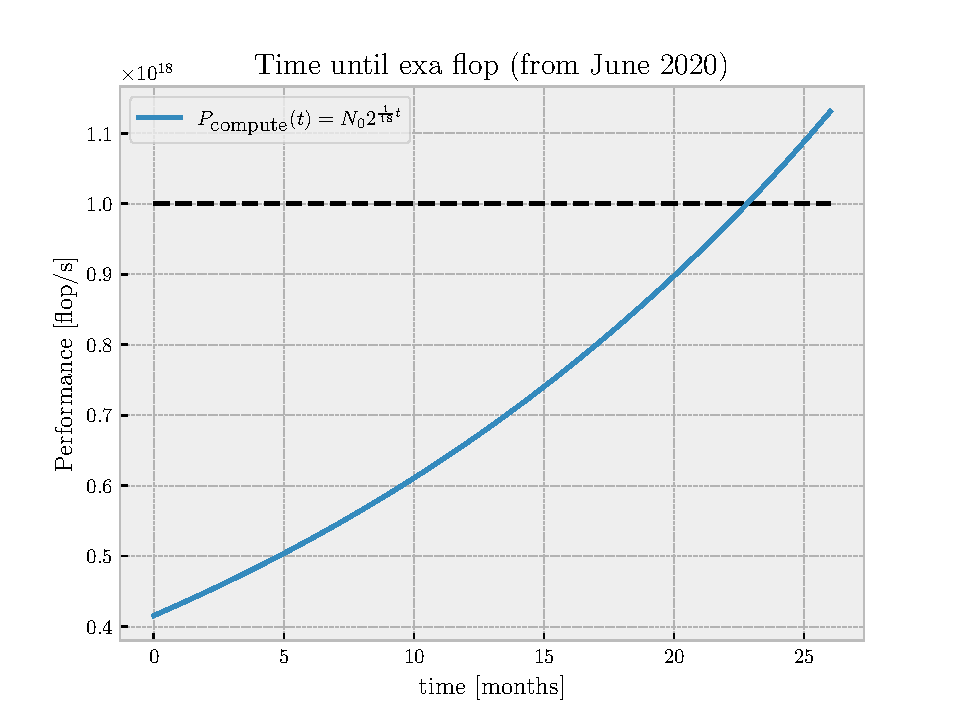
\includegraphics[width=0.8\linewidth]{./plots/Moore}
	\caption{Extrapolating time until exaflop from derived Moore's law}%
	\label{fig:Moore}
\end{figure}
\subsubsection{}
Determine time until exa scale from growth rate from TOP500 list
\begin{enumerate}
	\item Use data from 2007 and 2011
	\item Linear fit (on log scale) yields that exaflop performance should
		have been reached around 2018 (see figure~\ref{fig:GrowthRate})
\end{enumerate}
\begin{figure}[htpb]
	\centering
	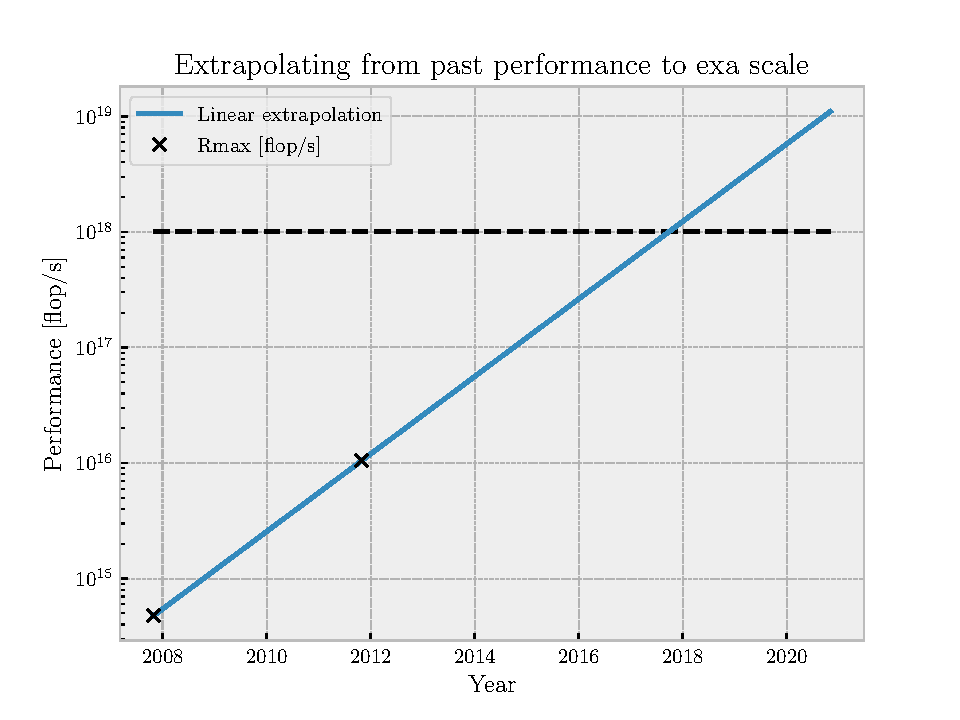
\includegraphics[width=0.8\linewidth]{./plots/GrowthRate.pdf}
	\caption{Extrapolating time until exaflop from TOP500 data using linear fit}%
	\label{fig:GrowthRate}
\end{figure}
$ \Rightarrow $ Extrapolating from past performance exaflop performance should have been
achieved around 2018, which is evidently not the case. Note however that extrapolation
from two data points is not very robust.

\newpage
\subsection{Amdahl's Law}
\subsubsection{}
\begin{itemize}
    \item new CPU 10 times faster
    \item old CPU spent 40\% of execution time on calculations
    \item remaining time was for IO
\end{itemize}
\begin{align}
    S &:= 60\%\\
    P &:= 40\%\\
    N &:= 10\\\nonumber\\
    Speedup &= \frac{1}{.6+\frac{.4}{10}} = 1.563
\end{align}

$\Rightarrow$ We would expect a 56\% performance improvement from the new CPU\@.

\subsubsection{}
\begin{itemize}
    \item 20\% of compute time is used for square roots
    \item possibilities:
        \begin{itemize}
            \item improve floating point square root calculations by factor of 10
            \item improve all FP operations by 1.6
        \end{itemize}
    \item 50\% of operation is spent on FP
\end{itemize}
\begin{align}
    S_1 &= \frac{1}{(1-(0.5\cdot 0.2))+\frac{0.5\cdot0.2}{10}}\\
        &= 1.099\\\nonumber\\
    S_2 &= \frac{1}{(1-0.5)+\frac{0.5}{1.6}}\\
        &= 1.231
\end{align}
$\Rightarrow$ By accelerating all FP operations by a facctor of 1.6 a speedup of 23\% can be observed and therefore is the optimal solution (in contrast to only 9.9\% when only speeding up FPSQRT).

\subsubsection{}
\begin{align}
    100 &= \frac{1}{(1-P)+\frac{P}{128}}\\
    \Leftrightarrow P&= 0.9978\\
    \Rightarrow S &\leq 0.22\%
\end{align}
\end{document}
